\chapter{Evaluation}\label{chap:Evaluation}
This section evaluates how successfully and effectively the implemented features achieve the goals stated in the introduction.

\section{Success}
This evaluation is more ambitious than that presented in the project proposal goals. As demonstrated below, the type witness search procedure and cast slicing features exceeds all core goals\footnote{That is, reasonable coverage and performance.} presented in the project proposal, while type slicing had not been conceived, but naturally complements cast slicing. Some extension goals were reached: almost of Hazel was supported\footnote{Except the type slicing of two constructs: type functions and labelled tuples (which was a new feature merged by the Hazel dev team in February).}. The search procedure was not mathematically formalised, but the slicing mechanisms were.

\section{Goals}\label{sec:EvaluationGoals}
This project devised and implemented three features: \textit{type slicing, cast slicing,} and a \textit{static type error witness search procedure}. Each of which had a clear intention for it's use:

\paragraph{Type Slicing:} Expected to give a greater static context to expressions. Explaining why an expression was given a specific type.

\paragraph{Cast Slicing:} Expected to provide static context to runtime type casts and propagate this throughout evaluation. Explaining where a cast originated and why it was inserted.

\paragraph{Search Procedure:} Finds dynamic type errors (cast errors) automatically, linked back to source code by their execution trace and \textit{cast slice}. Therefore, a static type error can be associated automatically with a concrete dynamic type error \textit{witness} to better explain.

\section{Methodology}\label{sec:EvaluationMethodology}
I evaluate the features and their various implementations (where applicable) along \textit{four} axes. With quantitative measures were evaluated over a corpus of ill-typed and dynamically-typed Hazel programs (\cref{sec:CorpusCollection}):

\subsubsection{Quantitative Analysis}
\paragraph{Performance: } \textit{Are the features performant enough for use in interactive debugging? Which implementations perform best?}

The time and space usage of the search procedure implementations were micro-benchmarked for each ill-typed program in the corpus. Up to 100 runs were taken per program with estimated time, major and minor heap allocations were estimated using an ordinary linear regression (OLS) via the \textit{bechamel} library \cite{Bechamel}.

\paragraph{Effectiveness: } \textit{Do the features effectively solve the problems? Are the results easily interpretable by a user?}

The \textit{coverage},  what proportion of programs admit a witness, for each search procedure implementation was measured. The search procedure does not always terminate, a 30s time limit was chosen. The coverage was expected to be \textit{reasonable}, chosen at 75\%.

Additionally, the \textit{size} of witnesses, evaluation traces, type slices, and cast slices were measured. The intention being that a smaller size implies that there is less information for a user to parse, and hence easier to interpret.\footnote{Not necessarily \textit{always} true, but a reasonable assumption.}

\subsubsection{Qualitative Analysis}
\paragraph{Critical: } \textit{What \textit{classes} of programs are missed by the search procedure? What are the implications of the \textit{quantitative} results? What improvements were, or could be made in response to these?}

This section provides \textit{critical} arguments on {usefulness} or {effectiveness}, which are \textit{evidenced} by quantitative data. Differing implementations and \textit{subsequent improvements}\footnote{Which were then implemented and analysed.} are compared. Additionally, further unimplemented improvements are proposed.

\paragraph{Holistic: } \textit{Do the features work well together to provide a helpful debugging experience? Is the user interface intuitive?}

Various program examples are given, demonstrating how all three features can be used together to debug a type error. Improvements to the UI are discussed.\footnote{Improved UI being a low-priority extension.} 



\section{Hypotheses}
Various hypotheses for properties of the results are expected. The evidence and implications of these are discussed in the \textit{critical evaluation}.

\paragraph{Search method space requirements: } The space requirements for DFS and Bounded DFS are expected to be lower than that of BFS and interleaved DFS.

\paragraph{Type Slices are larger than Cast Slices: } Casts are de-constructed during elaboration and evaluation, so cast slices are expected to be smaller than the original type slices, and therefore more directly explain why errors occur. 

\paragraph{The Small Scope Hypothesis: }
\label{sec:SmallScopeHypothesis} This hypothesis \cite{SmallScopeHypothesisOrigination} states that a high proportion of errors can be found by generating only \textit{small} inputs. Evidence that this hypothesis holds has been provided for Java data-structures \cite{SmallScopeHypothesis} and answer-set programs \cite{SmallScopeHypothesisAnswerSet}. Does it also hold for finding dynamic type errors from small \textit{hole instantiations}?

\paragraph{Smaller instantiations correlate with smaller traces: } As functional programs are often written recursively, destructuring compound data types on each step. If this and the small scope hypothesis hold, then most errors could be found with \textit{small execution traces}.

\section{Program Corpus Collection}\label{sec:CorpusCollection}

A corpus of small and mostly ill-typed programs was produced, containing both dynamic (unannotated) programs and annotated programs (containing statically caught errors). We have made this corpus available on GitHub \cite{HazelCorpus}.

\subsection{Methodology}
There are no extensive existing corpora of Hazel programs, nor ill-typed Hazel programs. Therefore, we opted to transpile parts of an existing OCaml corpus collected by Seidel and Jhala \cite{OCamlCorpus}. Which is freely available under a Creative Commons CC0 licence. 

I am grateful for my supervisor who created a best-effort OCaml to Hazel transpiler \cite{HazelOfOCaml}. This translates the OCaml examples into both a dynamic example, and a (possibly partially) statically typed version according to what type the OCaml type checker expects expression to be.\footnote{The annotations may be consistent, as we are translating ill-typed code.}

This corpus contains both OCaml unification and constructor errors. When translated to Hazel, these may manifest as differing errors. The only errors that the search procedure is expected to detect are those which contain \textit{inconsistent expectations} errors. Hence, the search procedure is ran on the corpus of annotated programs filtering those without this class of errors. Additionally, the search procedure requires the erroneous functions to have holes applied to start the search, these are inserted automatically by the evaluation code after type checking the programs.


\subsection{Statistics}
The program corpus contains \textbf{698} programs of which \textbf{203} were applicable to performing the search procedure on. Averages and standard deviations in size and trace size\footnote{When using normal, deterministic, evaluation.} shown in \cref{fig:CorpusStats}.
\begin{figure}
\centering
\begin{tabular}{c|ccccc}
& \textbf{Count} & \multicolumn{2}{c}{\textbf{Prog. Size}}& \multicolumn{2}{c}{\textbf{Trace Length}}\\
&  & Avg. & Std. dev. & Avg. & Std. dev.\\
\hline
\textbf{Unannotated} &404 &117 &81 &9&9\\
\textbf{Annotated} &294 &117 &76 &9&9\\
\textbf{Searched} &203 &120 &77 &10 &10\\
\hline
(Total)  &698 &117 &79 &9 &9\\
\end{tabular}
\caption{Hazel Program Corpus}
\label{fig:CorpusStats}
\end{figure}

\section{Performance Analysis}\label{sec:PerformanceAnalysis}

\subsection{Slicing}
The type and cast slicing mechanisms don't increase the time complexity of the type checker nor evaluator. Hence, they are still as performant as the original, capable of interactive use to medium sized programs.

\subsection{Search Procedure}
Only the annotated ill-typed corpus containing inconsistency errors are used in evaluating the search procedure. After all, any well-typed program cannot have a dynamic type error.

As the search procedure may be non-terminating, these results are found given a 30s time limit. Micro-benchmarking the programs which do not time-out, the time and space used searching for each witness can be estimated. 

The performance ratios between each implementation as compared to DFS on only the programs which \textit{both terminate} are given in \cref{fig:SearchPerformanceRatios}. As expected, BFS and IDFS use more memory in total than BDFS and DFS, while DFS is the fastest. 
\begin{figure}
  \centering
  \begin{tabular}{l|ccc}
  Ratios & \multicolumn{3}{c}{\textbf{Implementations}}\\
    vs. \texttt{DFS}& \texttt{BDFS} & \texttt{IDFS} & \texttt{BFS} \\
   \hline
   \textbf{Time} &  8.3 & 52 & 230\\
   \textbf{Major Heap} & 9.0 & 3.2 & 270\\
   \textbf{Minor Heap} & 9.7 & 83 & 390
  \end{tabular}
  
\caption{Benchmarks: Performance ratios to DFS over common programs}
\label{fig:SearchPerformanceRatios}
\end{figure}


\section{Effectiveness Analysis}\label{sec:EffectivenessAnalysis}


\subsection{Slicing}
\textit{Type slice} sizes (amount of highlighting) were calculated over the entire corpus. While \textit{cast slice} sizes were calculated over the resulting elaborated expressions.

\Cref{fig:TypeSlicingEffectiveness} shows that both type and cast slices are generally small. In particular, the proportion of the context\footnote{Calculated by close approximation by the \textit{program size}. As each program in the corpus is just one definition. Calculating the context itself is non-trivial.} highlighted is very low, generally less than 5\% for dynamic code and 10\% for annotated code. Therefore, they concisely explain the types.

Additionally, for errors, there will be multiple inconsistent slices involved. \Cref{sec:SlicingAnalysis} describes how these slices can be summarised to only report the inconsistent parts. We find that these \textit{minimised} error slices are significantly (3x) smaller than directly \textit{combining} the slices.

\begin{figure}[h]
  \centering
  \begin{tabular}{lc|c|ccc|ccc}
  \multicolumn{2}{c}{\textbf{Averages}} & \multicolumn{7}{c}{\textbf{Subdivisions}}\\
  & & & \multicolumn{3}{c|}{\textbf{Combined Error Slices}} & \multicolumn{3}{c}{\textbf{Minimised Error Slices}}\\ 
   & unit & ok & expects & branches & all & expects & branches & all\\
   \hline
   \textbf{Type Slice} & size &  8.2 & 13 & 22 & 15&  5.7 & 3.2 & 5 \\
   Std. dev. &  				 &  11 & 10 & 24 & 15&    4.31 & 4.1 & 4.4 \\
   \textbf{Proportion}& \%    & 5 & 8 & 14 & 9&        3  & 2 & 3 \\
   Std. dev. &  				 &  7 & 8 & 14 & 10&      3 & 3 & 3 \\
   \multicolumn{9}{c}{\textit{(Unannotated)}}\\
   \textbf{Type Slice} & size &  7.5 & 21 & 133* & 22.6 &8.2&  2.0* & 8.2  \\
   Std. dev. 			&    &  13 & 22 & 42* & 25.2& 12.6&  0.0* & 12.6  \\
   \textbf{Proportion}& \% 	 & 4 & 14 & 0.48* & 15&  6&    1* & 5  \\
   Std. dev. &  				 &  9 & 18 & 0.07* & 18&   9&    0* & 12  \\
   \multicolumn{9}{c}{\textit{(Annotated)}}\\
   \multicolumn{9}{c}{* only 2 annotated programs had inconsistent branches}
  \end{tabular}
  \caption{Effectiveness: Type Slices}
\label{fig:TypeSlicingEffectiveness}
\end{figure}
As hypothesised, combined slices within cast errors are smaller than combined static error slices on average (2x, \cref{fig:CastSlicingEffectiveness}). Therefore, casts can more precisely point to which part of an expressions type caused them.



\subsection{Search Procedure}

\subsubsection{Witness Coverage}
\begin{figure}[h]
\centering
\begin{subfigure}{0.45\textwidth}
\centering
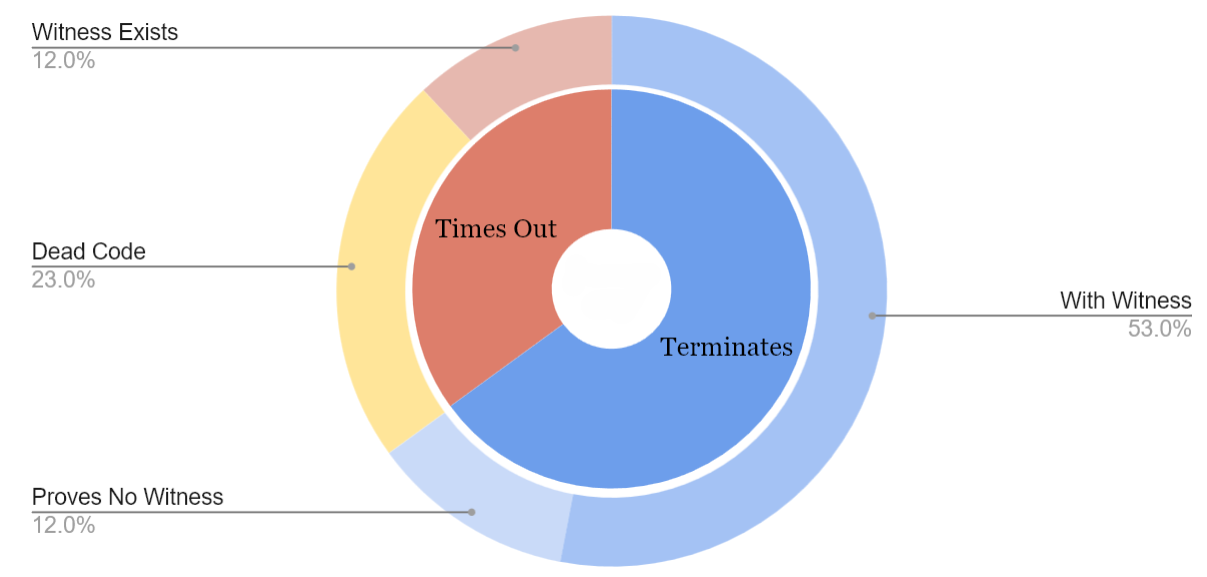
\includegraphics[width=1\textwidth]{Media/Figures/DFS_coverage}
\caption{DFS}
\end{subfigure}
%
\begin{subfigure}{0.45\textwidth}
\centering
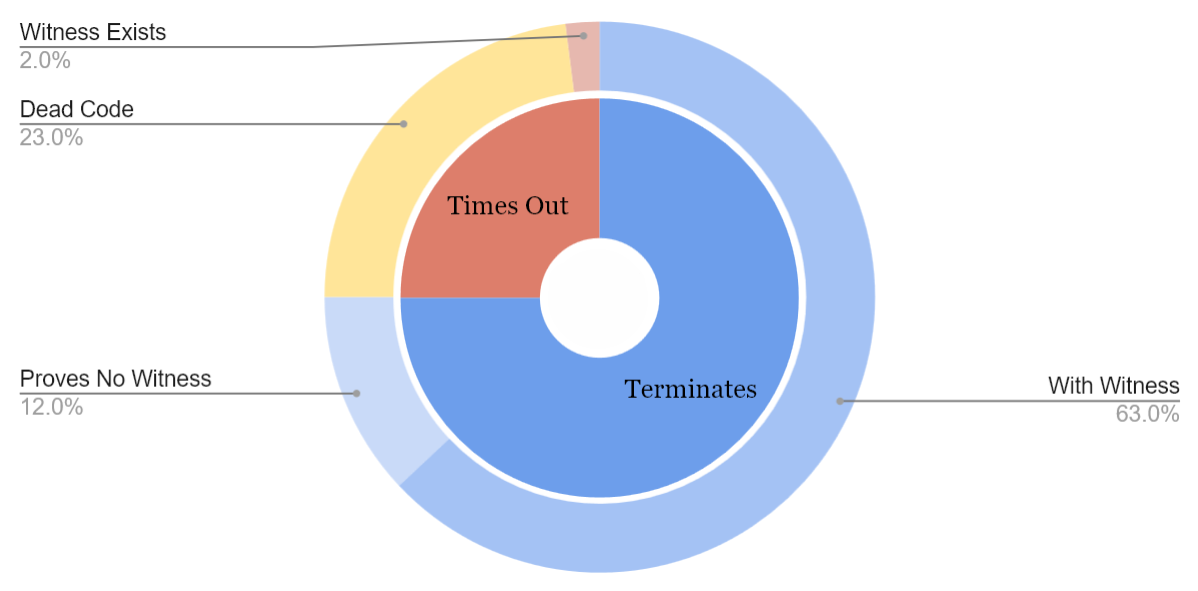
\includegraphics[width=1\textwidth]{Media/Figures/BDFS_coverage}
\caption{Bounded DFS}
\end{subfigure}

\vspace{1cm}

\begin{subfigure}{0.45\textwidth}
\centering

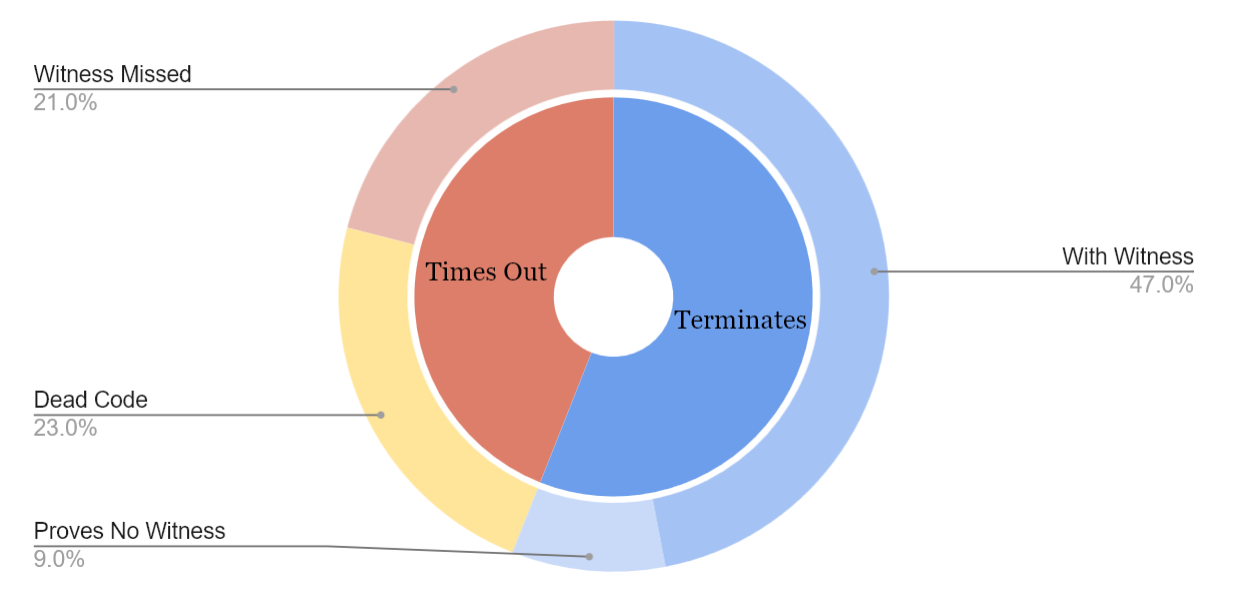
\includegraphics[width=1\textwidth]{Media/Figures/IDFS_coverage}
\caption{Interleaved DFS}
\end{subfigure}
%
\begin{subfigure}{0.45\textwidth}
\centering

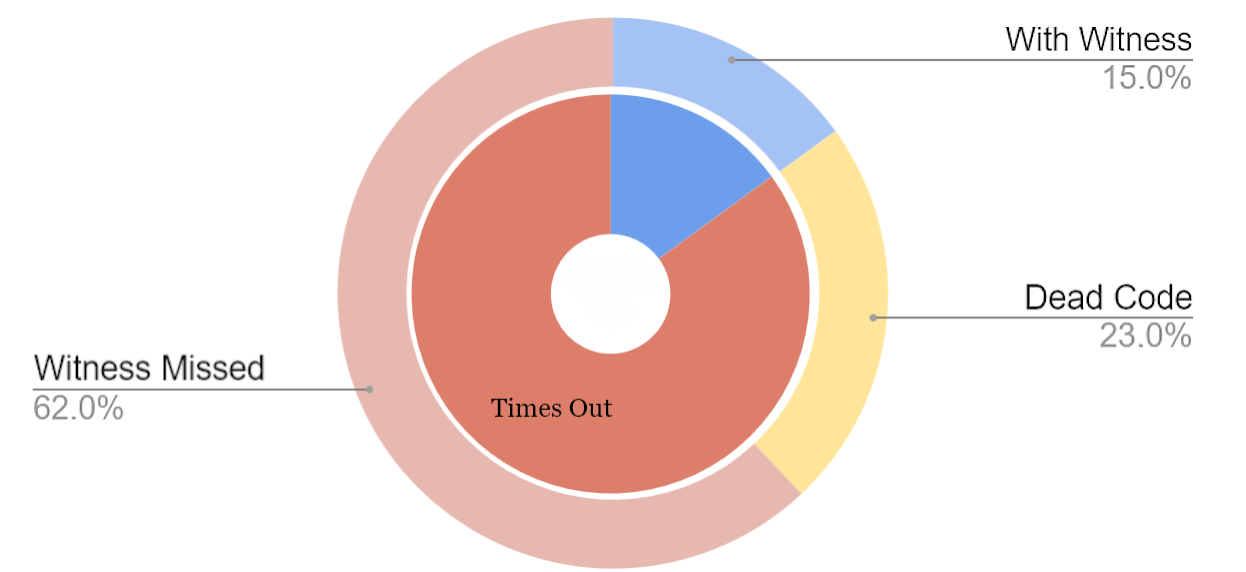
\includegraphics[width=\textwidth]{Media/Figures/BFS_coverage}
\caption{BFS}
\end{subfigure}

\caption{Search Procedure Coverage}
\label{fig:PieChart}
\end{figure}

The search procedure terminates either with a witness or proving no witness exists. A majority of programs terminated when using BDFS, DFS and IDFS, with BDFS meeting the 75\% target directly (\cref{fig:PieChart}). IDFS and BFS perform relatively poorly likely due to excessive memory usage (\cref{fig:SearchPerformance}). 

However, not all static errors have a dynamic witness, e.g. errors within dead code. I manually classified each failed program for BDFS to check if a witness does exist, but was not found, or no witness exists. This gives only 2\% of cases where BDFS failed to actually find an \textit{existing} witness; DFS and IDFS also meet the goal of failing in less than 25\% of cases. \Cref{sec:SearchCategories} goes into further detail on categorising the programs which time out, and how this could be avoided.

\subsubsection{Witness \& Trace Size}
As predicted by the small-scope hypothesis, most programs admitted \textit{small} witnesses (avg. sizes of 1-2, i.e. mostly base cases). 

However, there was no linear correlation (Pearson correlation coefficient $= 0$) between witness sizes and trace sizes, even when normalised by the original deterministic evaluation trace lengths. This is likely because most errors are in the base cases, so few large witnesses are even found, with the noise from trace lengths to different programs' base cases dominating. 



\section{Critical Analysis}\label{sec:CriticalAnalysis}
This section discusses the implications of the previous results and delves deeper into the reasoning behind them. As a response to this analysis, many improvements have been devised, some of which have been implemented.
\subsection{Slicing}\label{sec:SlicingAnalysis}
Type slicing theory (\cref{sec:TypeSlicingTheory}) requires highlighted code to form valid expressions or contexts, though some highlighted parts, like unused or dynamic bindings, don't affect types and can be omitted. This motivated the use of unstructured (ad-hoc) slices (\cref{sec:UnstructuredSlices}).

In \cref{fig:LetSliceOmitted}, a bound integer \code{x} is only used in one branch. Since the other branch can already determine the type of the conditional, the $\code{x}$  and \code{let} are excluded from the slice. Though the whole program is selected,\footnote{See the red cursor.} the let expression is omitted. A contribution slice would include everything,\footnote{Both branches must be shown, as \code{x} needs to type-check.} making it even more verbose.
\begin{figure}
\centering
\begin{subfigure}{0.45\textwidth}
\centering

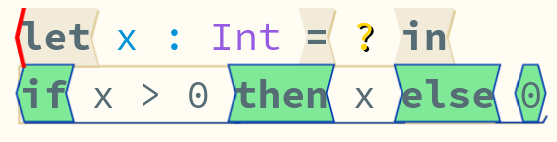
\includegraphics[width=0.85\textwidth]{Media/Figures/Unused_let}
\caption{Ad-hoc Slice: Let expression omitted}
\end{subfigure}$\qquad$
\begin{subfigure}{0.45\textwidth}
\centering

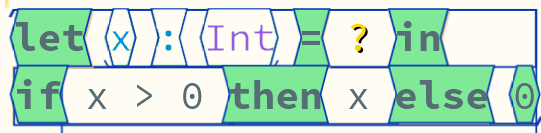
\includegraphics[width=0.85\textwidth]{Media/Figures/Unused_let_ordinary}
\caption{Ordinary Slice}
\end{subfigure}

\caption{An Ad-hoc Slice vs. Ordinary Slice}
\label{fig:LetSliceOmitted}
\end{figure}


\subsubsection{Error Slices}
\label{sec:ErrorSlices}
Type errors arise from inconsistencies between a term’s analysis and synthesis slices, or across synthesising branches. Understanding the error requires comparing all the slices involved.

Some type parts may agree, hence another form of type joining was introduced to isolate only the inconsistent parts. For instance, in \cref{fig:ErrorSlice}, differences like \code{(Int, Int)} vs \code{(Int, String)} highlight only the mismatched sub-slices.

\begin{figure}[h]
\begin{subfigure}{0.45\textwidth}
\centering

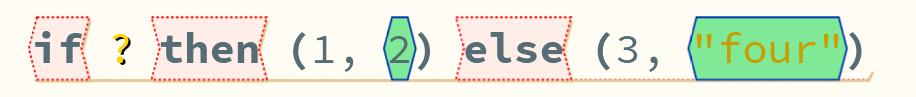
\includegraphics[width=1\textwidth]{Media/Figures/partially_inconsistent_branches}
\caption{Partially Inconsistent Branches}
\end{subfigure}$\qquad$
\begin{subfigure}{0.45\textwidth}
\centering

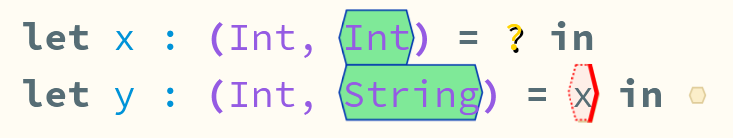
\includegraphics[width=1\textwidth]{Media/Figures/partially_inconsistent_expectations}
\caption{Partially Inconsistent Expectations}
\end{subfigure}

\caption{Error Slices}
\label{fig:ErrorSlice}
\end{figure}

Compound type inconsistencies necessarily differ at the outermost constructor (e.g., \code{List} vs \code{Int}), being the \textit{primary} cause of the error. Deeper inconsistencies are not those causing the type error. Therefore, we could extract only the slice on the outermost constructor. These minimised slices (\cref{fig:MinimisedSlice}) are significantly (avg. 3x) smaller than full combined slices (\cref{fig:TypeSlicingEffectiveness}). This ratio may grow with program complexity.\footnote{The dataset had few partially inconsistent cases, where the biggest savings occur.}

\begin{figure}[h]
\centering
\begin{subfigure}{0.3\textwidth}
\centering

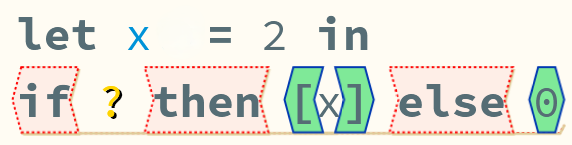
\includegraphics[width=1\textwidth]{Media/Figures/partially_inconsistent_compound}
\caption{Minimised Error Slice: Inner \code{Int} slice within list is omitted}
\end{subfigure}$\qquad\qquad$
\begin{subfigure}{0.3\textwidth}
\centering

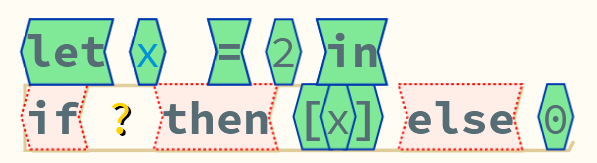
\includegraphics[width=1\textwidth]{Media/Figures/partially_inconsistent_compound_ordinary}
\caption{Ordinary Error Slice}
\end{subfigure}

\caption{Minimised Error Slices}
\label{fig:MinimisedSlice}
\end{figure}

\subsection{Structure Editing}\label{sec:StructureEditing}
Hazel uses a structure editor with an update calculus \cite{HazelStructureCalculus}, where statics are recalculated on edits, even cursor movement. While slice-based type checking is fast, it's less ideal for such interactive use in large programs.

Hazel ensures efficient edits\footnote{In constant time.} via a zipper data structure \cite{Zipper, OneHoleContext}. Extending this to the AST and typing info could enable edits to only locally update the type  information. However, some edits (e.g. adding a binding) can cause non-local, more extensive, type recalculation, but, these are rare. Such a system would require a major rewrite of Hazel's statics, with benefits beyond just type slicing.
  
\subsection{Static-Dynamic Error Correspondence}
\label{sec:ErrorCorrespondence}

A static type error will place a term inside a cast error during elaboration, which can be associated with a dynamic error whose cast error is dependent on (decomposed from) this original failed cast. This works well for \textit{inconsistent expectations} static type errors.

However, for inconsistent branches, no direct cast failure occurs until both are evaluated in a shared static context. The search might find such cases, but linking them back to the static error is harder. Still, since elaboration adds casts to each branch, these can be tracked with the error.\footnote{But we cannot assume the inconsistent branches caused the error; it might instead be the context using the value that is incorrect.}
  
\subsection{Categorising Programs Lacking Type Error Witnesses}
47 programs which timed out under the BDFS search procedure were manually inspected and classified as either:
\begin{itemize}
\item Witness Exists: BDFS failed to find an existing witness.
\item Dead Code: The error lies in unreachable code:
\begin{itemize}
\item Pattern Cast Failure: Error within a pattern matching branch, making the branch unreachable. These are detectable by the extended pattern directed instantiation algorithm (\cref{sec:ExtendedPatternMatching}).\footnote{The inconsistent patterns would be attempted, and subsequently reduced to expression cast failures.}
\item Unbound Constructor: Attemping to match an unbound constructor. Also detectable with the extended instantiation.
\item Wildcards: Erroneous code bound to the inaccessible wildcard pattern: \code{let _ = ... in ...}.
\item Non-Trivial: Less easily detectable. One example exhibited this, infinitely recursing for all inputs.
\end{itemize}
\item Hazel Bugs: Unboxing bugs present in the main branch (excluded from the statistics).
\end{itemize}
\Cref{fig:FailureDistribution} shows this distribution and three (paraphrased) examples are given in the appendix \cref{fig:FailureExamples}. The full classification is in \texttt{failure-classification.txt}.

\begin{figure}[h]
\centering
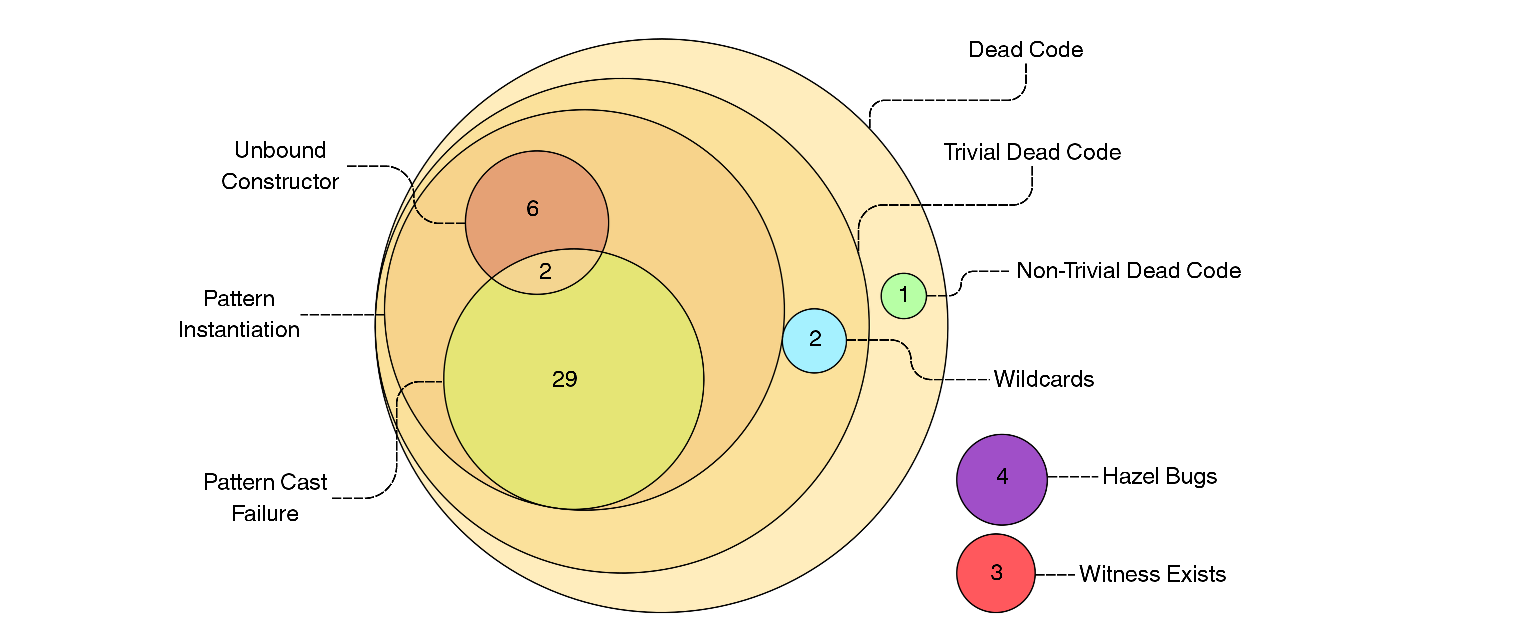
\includegraphics[width=1\textwidth]{Media/Figures/Failures}
\caption{Distribution of Failed Program Classes}
\label{fig:FailureDistribution}
\end{figure}

\label{sec:SearchCategories}
\subsubsection{Non-Termination, Unfairness, and Search Order}
DFS is fast but prone to non-termination, giving it lesser coverage than BDFS (\cref{fig:PieChart}). If evaluation infinitely loops, so will DFS without exploring other instantiations. It is also unfair, it may never try some instantiations \cite{FairNondeterminism}. This affected 10\% of cases.

To address this, BDFS, BFS, and IDFS were implemented, with BDFS performing the due to prioritising evaluation over instantiation. BFS and IDFS would do significantly better if they tried longer trace length more frequently, on average reaching only half the trace length (full data: \cref{fig:WitnessSize}). Wrapping evaluation in the evaluation algorithm would help this, but choosing how frequently to wrap evaluation is a delicate balancing act.

\subsubsection{Dead Code \& Nested Errors}

Errors within dead code cannot have a witness as they are not dynamically reachable. A significant portion (39/47) of failed programs for BDFS had trivial dead code which could easily be detected and returned explicitly as proving no witness exists.

Additionally, code can become dead due to errors. 12 (32\%) of the dead code classified had a nested error within a branch that is unreachable due to a pattern error on the branch pattern. Even if witnesses are found for these branch errors, the nested errors remain hidden.

\subsubsection{Dynamically Safe Code}
Some static errors is inherently dynamically safe, having no witness, e.g. \code{if true then 0 else "str"}. The search procedure often proves this by running out of instantiations: BDFS proved no witness 12\% of the time. 

However, in general, safe code may lead to non-terminating searches, endlessly generating witnesses. So, a timeout does not necessarily imply a witness was found, or that none exist.

\subsubsection{Cast Laziness}\label{sec:EvalCastLaziness}
Hazel treats casts lazily, deferring cast transitions on compound data until their elements are used (e.g., tuple elements). Hazel does not detect cast errors between these non-ground compound types (e.g., \code{[Int]} vs \code{[String]}) until elements are used. Therefore if such elements are unused in code, the error cannot be witnessed. These are uncommon, none appearing in the search corpus.

Addressing this would require eager cast semantics, as has been previously explored for dynamic and gradual type systems \cite{EagerCasts, GradualEagerCasts}.\footnote{Often referred to as coercions.} Additionally, they would catch dynamic errors earlier, for example, \cref{fig:LazyCastError} shows a cast inconsistency undetected (by lazy casts) at runtime until the tuple element is accessed.
\begin{figure}[h]
\centering
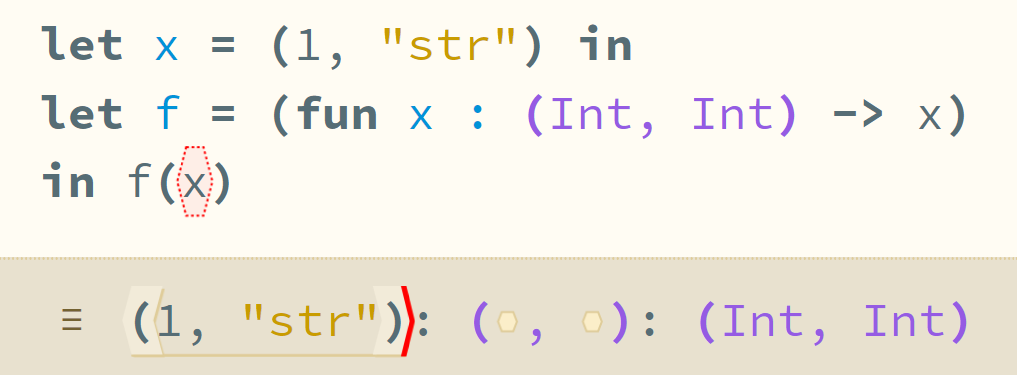
\includegraphics[width=0.4\textwidth]{Media/Figures/cast_laziness_no_error}
\caption{Inconsistent Lazy Casts: No Cast Failure}
\label{fig:LazyCastError}
\end{figure}

\subsubsection{Combinatorial Explosion}
When multiple holes are involved in searching, the search space increases exponentially. This combinatorial explosion especially impacts IDFS and BFS, who prioritise instantiation over evaluation. This leads to high memory use and hinders evaluation from progressing far enough to detect errors, even when valid witnesses have been instantiated.

Further, some errors only arise on very specific inputs, e.g. \code{(23, 31)} and \code{(31, 23)} in \cref{fig:SpecificInstantiations}. Directing instantiation to maximise code coverage earlier could find such errors attempting fewer instantiations.
\begin{figure}\centering
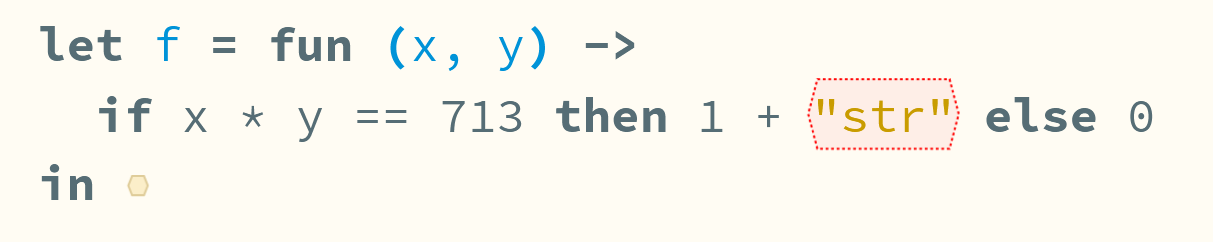
\includegraphics[width=0.6\textwidth]{Media/Figures/very_specific_error}
\caption{Witness Requiring Very Specific Instantiations}
\label{fig:SpecificInstantiations}
\end{figure}

\subsection{Improving Code Coverage}
\label{sec:EvalHoleInstantiation}
The search procedure struggles when compound witnesses require specific, interdependent parts, being much less likely to instantiate. These errors are also harder for programmers to detect or understand; understanding the error might require recognizing input interdependencies.

Intelligently directing hole instantiations to better cover the code would help. A pattern-directed instantiation as described in \cref{sec:ExtendedPatternMatching} would discover 2 of the 3 missed witnesses by BDFS.

Still, BDFS retains a very high coverage over the search procedure when excluding dead code (97\%).

\section{Holistic Evaluation}
\label{sec:HolisticEvaluation}

This section considers a number of examples of ill-typed Hazel programs, \textit{holistically} and \textit{qualitatively} evaluating how a user might use the three features and the existing bidirectional type error localisation \cite{MarkedLocalisation} to debug the errors. 


\subsection{Interaction with Existing Hazel Type Error Localisation}
Hazel has three error types addressed by this project:\footnote{Other errors: syntax errors, unbound variables, label errors etc. are out of scope} \textit{inconsistent expectations} (analytic and synthetic types are inconsistent), \textit{inconsistent branches }(branches or list element types are inconsistent), and \textit{inexhaustive matches}. 

\Cref{sec:ErrorCorrespondence} showed how witnesses can be associated to inconsistency errors. While indeterminate evaluation can give examples for pattern inexhaustivity, standard pattern matrix methods \cite{PatternMatchingWarnings} are more efficient.\footnote{The matrices also useful for directing pattern instantiation}

When errors arise from the programmer \textit{misunderstanding} the program types, error localisation can be inaccurate (due to assuming different types to the programmer's expectations). The context inspector (\cref{fig:ContextInspector}) clarifies what assumptions the system makes while slicing and witnesses can explain \textit{why}.

\begin{figure}[h]\centering
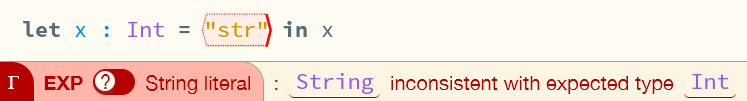
\includegraphics[width=0.7\textwidth]{Media/Figures/context_inspector}
\caption{Selected Static Error described by Hazel Context Inspector}
\label{fig:ContextInspector}
\end{figure}

When the programmer and system agree on the types, bidirectional typing generally localises the error(s) well \cite{BidirectionalTypes, MarkedLocalisation}. However, there is not always enough static information to even recognise errors, and many type annotations may need to be inserted to detect the error. The search procedure tests such code for such type errors automatically, and can be a quicker way to detect these errors than adding annotations. 

\subsection{Examples}
\label{sec:EvalExamples}

\begin{figure}[h]
\centering
\begin{subfigure}{0.49\textwidth}
\centering
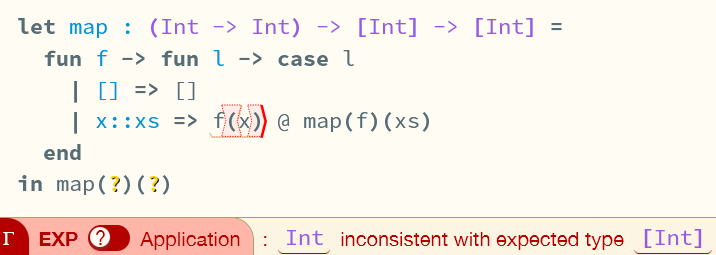
\includegraphics[width=1\textwidth]{Media/Figures/map_example}
\caption{Error}
\end{subfigure}
\begin{subfigure}{0.49\textwidth}
\centering
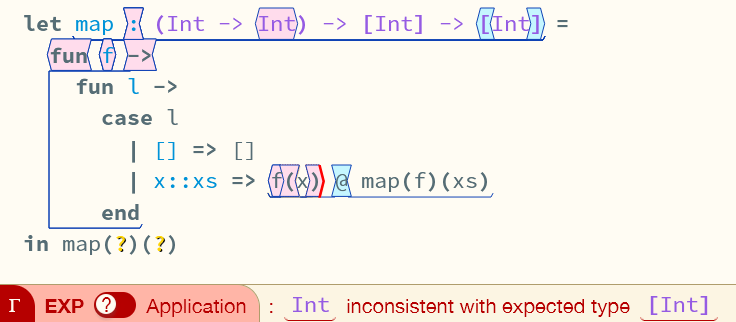
\includegraphics[width=1\textwidth]{Media/Figures/map_example_sliced}
\caption{With Error Slice}
\end{subfigure}
\caption{Inconsistent Expectations: \code{f(x)} synthesises type \code{Int} but analyses against \code{[Int]}. The \textit{minimised} error slice shows (in pink) why \code{Int} is synthesised (due to input \code{f} being annotated \code{Int -> Int} and applied) and (in blue) why a list is expected.}
\label{fig:MapExample}
\end{figure}
\begin{figure}[h]
\centering
\begin{subfigure}{0.4\textwidth}
\centering
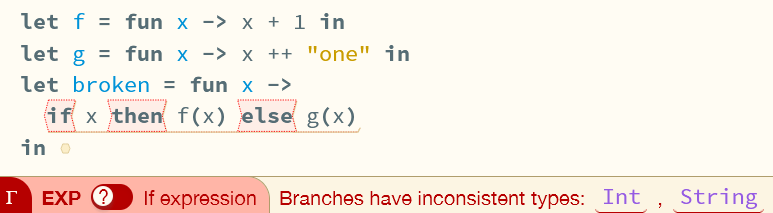
\includegraphics[width=1\textwidth]{Media/Figures/inconsistent_branches_example}
\caption{Error}
\end{subfigure}$\qquad$
\begin{subfigure}{0.4\textwidth}
\centering
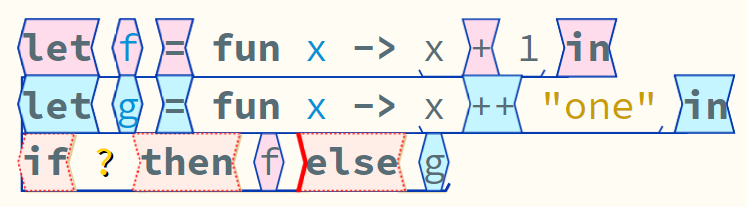
\includegraphics[width=1\textwidth]{Media/Figures/inconsistent_branches_example_sliced}
\caption{With Error Slice}
\end{subfigure}
\caption{Inconsistent Branches: A more complex inconsistency involving non-local bindings. \textit{Minimal} error slices highlight only the bindings, and conflicting addition and string concatenation operators.}
\label{fig:InconsistentBranchesExample}
\end{figure}

{\begin{figure}[H]
\centering
\begin{subfigure}[t]{0.49\textwidth}
\centering
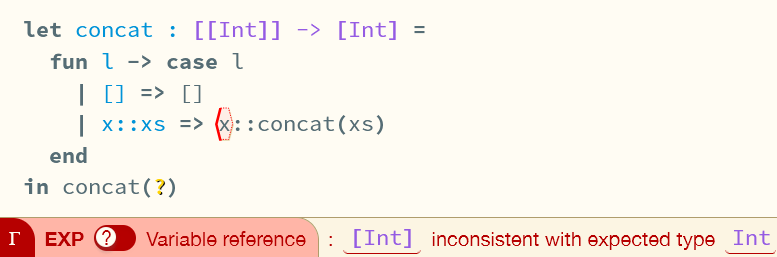
\includegraphics[width=1\textwidth]{Media/Figures/concat_error}
\caption{The user thinks that list cons \code{::} concatenates lists.}
\end{subfigure}
\begin{subfigure}[t]{0.49\textwidth}
\centering
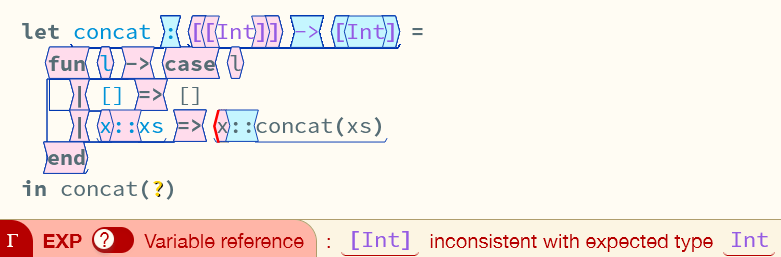
\includegraphics[width=1\textwidth]{Media/Figures/concat_error_type_slice}
\caption{Error slice highlights the offending \code{::}, but with considerable noise distracting from this. Also, if the user still expects \code{::} to perform concatenation, this is useless.}
\end{subfigure}
\begin{subfigure}{0.49\textwidth}
\centering
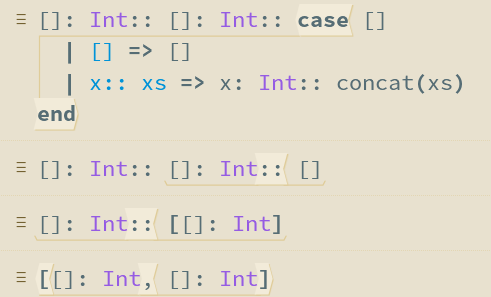
\includegraphics[width=1\textwidth]{Media/Figures/concat_error_trace}
\caption{The user cycles through increasingly larger witnesses (until \code{[[], []]}) to spot the consing pattern. End of trace concretely shows \code{::} acting as cons.}
\end{subfigure}
\begin{subfigure}{0.49\textwidth}
\centering
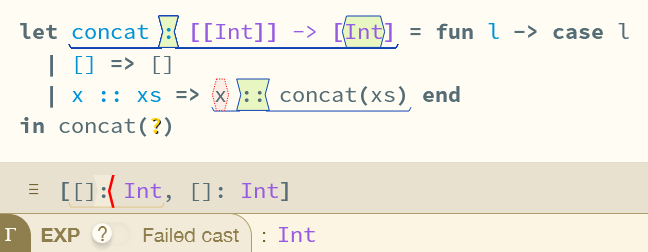
\includegraphics[width=1\textwidth]{Media/Figures/concat_error_cast_slice}
\caption{Alternatively, the cast slice to \code{Int} concisely retrieves the relevant part of the original type slice.}
\end{subfigure}
\caption{Holistic Example involving all three features}
\label{fig:ConcatError}
\end{figure}}

\begin{figure}[h]
\begin{subfigure}{0.49\textwidth}
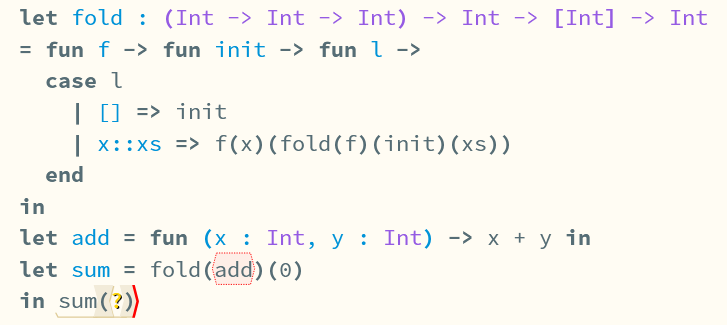
\includegraphics[width=1\textwidth]{Media/Figures/curries}
\caption{Fold takes curried functions, but uncurried add is used.}
\end{subfigure}
\begin{subfigure}{0.49\textwidth}
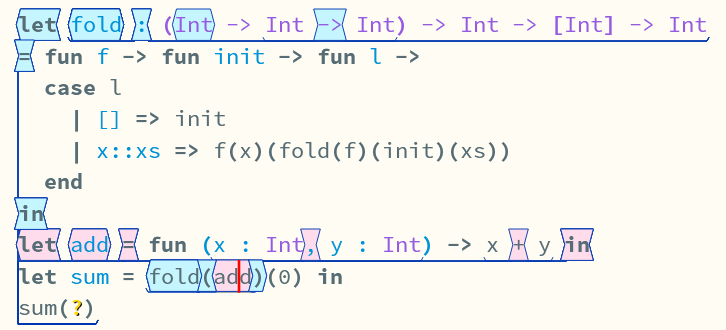
\includegraphics[width=1\textwidth]{Media/Figures/curries_type_slice}
\caption{Error slice is verbose, and merges multiple inconsistencies: $\code{(Int, Int)} \not\sim \code{Int}$ and $\code{Int} \not\sim \code{Int} \to \code{Int}$. The second inconsistency is minimised to $\code{Int} \not\sim \dyn \to \dyn$.}
\end{subfigure}
\begin{subfigure}{0.49\textwidth}
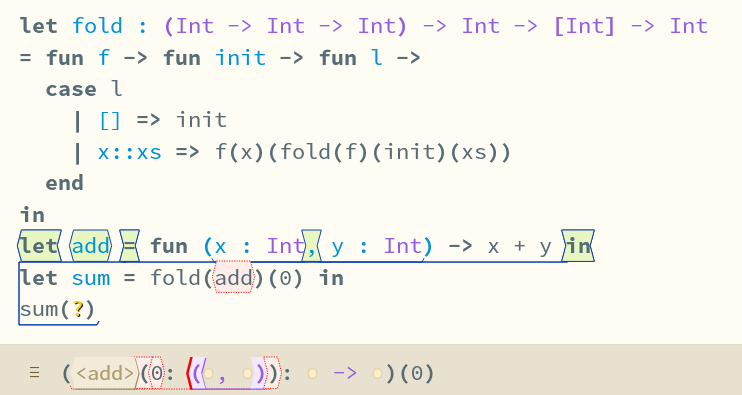
\includegraphics[width=1\textwidth]{Media/Figures/curries_expects_tuple}
\caption{Witness (\code{[0]}) found automatically: expects input $0$ into \code{add} to be a tuple. Cast slice considers only the $\code{(Int, Int)} \not\sim \code{Int}$ inconsistency.}
\end{subfigure}
\begin{subfigure}{0.49\textwidth}
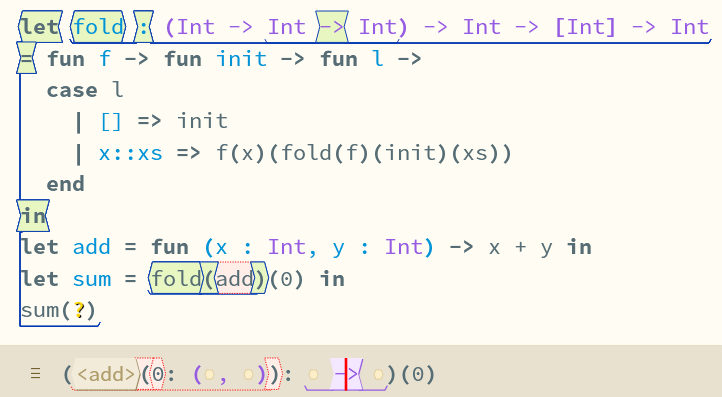
\includegraphics[width=1\textwidth]{Media/Figures/curries_expects_function}
\caption{Same witness has a second cast error: output of \code{add(0)} is expected to be a function. Cast slice considers only the minimised $\code{Int} \not\sim {\dyn \to \dyn}$ inconsistency.}
\end{subfigure}
\caption{A more subtle holistic example involving currying. Requires slice decomposition internally.}
\label{fig:TastyCurry}
\end{figure}

\begin{figure}[h]
\centering
\begin{subfigure}{0.45\textwidth}
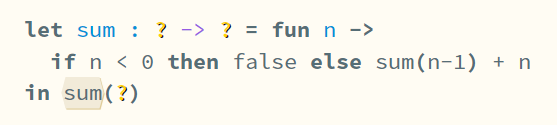
\includegraphics[width=1\textwidth]{Media/Figures/dynamic_code_error}
\caption{Error}
\end{subfigure}
\begin{subfigure}{0.45\textwidth}
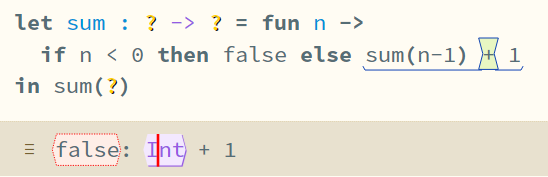
\includegraphics[width=1\textwidth]{Media/Figures/dynamic_code_error_cast_slice}
\caption{Automated witness found with cast slice blaming \code{+} operator}
\end{subfigure}
\caption{Dynamic Code: An error is not statically found. Cast slicing still works even without the type annotations, blaming addition forcing ints.}
\label{fig:DynamicExample}
\end{figure}